%--------|---------|---------|---------|---------|---------|---------|---------|
%       10        20        30        40        50        60        70        80
%-------------------------------------------------------------------------------



\documentclass[11pt, twoside, titlepage, a4paper]{article}
% set utf8 encoding, and set font encoding T1 to allow "|" ">" "<" etc
\usepackage[utf8]{inputenc}
\usepackage[T1]{fontenc}
\usepackage[a4paper,inner=40mm,outer=25mm,top=25mm,bottom=25mm,pdftex]{geometry}
% These page settings give images 1.0\linewidth around 135-140mm wide (ca 138mm)
% meaning a 300dpi image is around 1600 pixels wide
\usepackage{graphicx}   % For eps figures
\usepackage{epsfig}     % Alternative package
\usepackage[hang,small,bf]{caption}

\usepackage[british]{babel}       

\usepackage[yyyymmdd]{datetime}
\renewcommand{\dateseparator}{--}

\usepackage{fancyhdr}
\pagestyle{fancy}
% with this we ensure that the chapter and section
% headings are in lowercase.
%\renewcommand{\chaptermark}[1]{\markboth{#1}{}}  % no "\chapter" in article doc type
\renewcommand{\sectionmark}[1]{\markright{\thesection\ #1}}
\fancyhf{} % delete current setting for header and footer
\fancyhead[LE,RO]{\bfseries\thepage}
\fancyhead[LO]{\bfseries\rightmark}
\fancyhead[RE]{\bfseries\leftmark}
\renewcommand{\headrulewidth}{0.5pt}
\renewcommand{\footrulewidth}{0pt}
\addtolength{\headheight}{0.5pt} % make space for the rule
\fancypagestyle{plain}{%
    \fancyhead{} % get rid of headers on plain pages
    \renewcommand{\headrulewidth}{0pt} % and the line
}


% remove forced implicit vertical whitespace before and after verbatim environment
\makeatletter
\preto{\@verbatim}{\topsep=0pt \partopsep=0pt }
\makeatother


% allow to force indentation of first line in section
% \indent is not working, so workaround \hspace{\parindent} works
\newcommand{\forceindent}{\hspace{\parindent}}


\newcommand{\degrees}{$^\circ$~}
\newcommand{\degree}{$^\circ$}
\newcommand{\ca}{$\approx$}

\newcommand{\vs}{$\backslash\ $}  % "versus" slash
\newcommand{\bs}{$\backslash\ $}  % just backslash


% want clear dash insert commands
\newcommand{\dash}{-}     % just a normal hyphen dash  "-"
\newcommand{\ndash}{--}   % n-dash "--"
\newcommand{\mdash}{---}  % m-dash "---"


%link new command names to the original font sizes,
%for easier to remember smaller font size
\newcommand{\vsmall}{\footnotesize}  % simpler to remember
\newcommand{\vvsmall}{\scriptsize}   %
%\newcommand{\vvvsmall}{\tiny}


\usepackage[colorlinks=true,linkcolor=black,urlcolor=blue]{hyperref}


\usepackage{ifthen}


% \needspace{5\baselineskip}      << reserves approximately 5 lines, leaves raggedbottom, more efficient
% \Needspace{5\baselineskip}      << reserves exactly 5 lines, leaves raggedbottom, less efficient
% \Needpsace*{5\baselineskip}     << leaves flushbottom if \flushbottom is in effect, otherwise ragged
\usepackage{needspace}



% \skill{blabla}
\newboolean{skillsaslist}
\setboolean{skillsaslist}{true}
\ifthenelse{\boolean{skillsaslist}}{\newcommand{\skill}[1]{\item[#1]}}{\newcommand{\skill}[1]{\subsubsection*{#1}}}
\ifthenelse{\boolean{skillsaslist}}{\newcommand{\openskillslist}{\begin{description}}}{\newcommand{\openskillslist}{}}
\ifthenelse{\boolean{skillsaslist}}{\newcommand{\closeskillslist}{\end{description}}}{\newcommand{\closeskillslist}{}}

% \action{blabla}
\newboolean{actionsaslist}
\setboolean{actionsaslist}{true}
\ifthenelse{\boolean{actionsaslist}}{\newcommand{\action}[1]{\item[#1]}}{\newcommand{\action}[1]{\subsubsection*{#1}}}
\ifthenelse{\boolean{actionsaslist}}{\newcommand{\openactionslist}{\begin{description}}}{\newcommand{\openactionslist}{}}
\ifthenelse{\boolean{actionsaslist}}{\newcommand{\closeactionslist}{\end{description}}}{\newcommand{\closeactionslist}{}}

% \eqitem{blabla}
\newboolean{itemsaslist}
\setboolean{itemsaslist}{true}
\ifthenelse{\boolean{itemsaslist}}{\newcommand{\eqitem}[1]{\item[#1]}}{\newcommand{\eqitem}[1]{\subsubsection*{#1}}}
\ifthenelse{\boolean{itemsaslist}}{\newcommand{\openitemslist}{\begin{description}}}{\newcommand{\openactionslist}{}}
\ifthenelse{\boolean{itemsaslist}}{\newcommand{\closeitemslist}{\end{description}}}{\newcommand{\closeactionslist}{}}


\newenvironment{readoutloud}%
{\begin{quote}\begin{itshape}}%
{\end{itshape}\end{quote}}%



% need a nice easily visible TODO marker
\newcommand{\todo}{\textbf{TODO:}~}
\newcommand{\TODO}{\LARGE\textbf{TODO:}\normalsize~}







%-------------------------------------------------------------------------------
\begin{document}


% too many words in common across docs nowadays
%--------|---------|---------|---------|---------|---------|---------|---------|
%       10        20        30        40        50        60        70        80
%-------------------------------------------------------------------------------


% Manually specify hyphenation for names.
% Remember: space separated word list: lead with space
% hyphens can only occur on specified "-" characters
% words without "-" will never be hyphenated, overrides language rules
\hyphenation{
 cam-paign-ab-il-ity
 Thing-a-ma-jig
 milli-fort-night
 Kings-land
 Evil-nius Conq
 Massa Pawa
 Maj-san Go-san Mal-vi-na
 Ho-her
 Bea-ta Blo-dig
 Leg-io Legu-ano
 Gammel-Tant
 Gam-ling
 Hem-ske-lina
 Go-blan-da
 Stur-Skurk
 Hjal-mar Hjäl-te
 Bur-mak
 Lund-qvist
 Grim-Gnash
 Gros-Orc
 muta-mon-ster
 muta-meat
 Iffy-Griff
 Hoo-man Hoo-mans hoo-man hoo-mans
 Da-ta-ri-an Ma-ras No-stro-mo
 Uchly Namen
 Edwin Chro-mo-phobe
 Star-Craft Brood War Brood-War
 Space Hulk
 Hermann Hammer-hand
}




%-------------------------------------------------------------------------------
% title page
%-----------


\thispagestyle{empty}

\null          % make an empty mark, so that following white space will be honoured
\vspace{1cm}   % not honoured at beginning of page without something above

\begin{center}

\huge
Turn Off the Light

\vspace{0.3\baselineskip}

\large
How many Heroes does it take to unscrew a light bulb?\\
How many will die in the process?

\vspace{2cm}

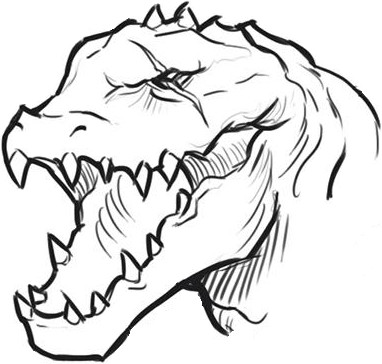
\includegraphics[width=80mm]{./fig/lizardman-head.jpg}

\vspace{2 cm}


\normalsize
under construction\\
major blanks

\vfill

\today

\end{center}






%-------------------------------------------------------------------------------
% copyright etc on the back side of the title page
%-------------------------------------------------
\clearpage
\thispagestyle{empty}
\raggedbottom

\vsmall
\noindent
This work is licensed under a Creative Commons \\
Attribution-NonCommercial-ShareAlike 4.0 \\
International License. (CC BY-NC-SA 4.0).\\
\url{https://creativecommons.org/licenses/by-nc-sa/4.0/} \\
\url{https://creativecommons.org/licenses/by-nc-sa/4.0/legalcode} \\
If you want to use it in any other fashion please contact the author.

\

\noindent
All images are temporary placeholders, \\
most are downloaded and unattributed.\\
They need to be replaced with licensed art.

\normalsize






%-------------------------------------------------------------------------------
% begin main matter
%------------------
\cleardoublepage
\pagestyle{fancy}
%\flushbottom
\raggedbottom




%--------|---------|---------|---------|---------|---------|---------|---------|
%       10        20        30        40        50        60        70        80
%-------------------------------------------------------------------------------
\phantomsection\addcontentsline{toc}{section}{Turn Off the Light}
\section*{Turn Off the Light}

The Heroes are hired to destroy a magical power focus, deep in a cave warren, guarded by dangerous well trained lizard men.
They will be teleported deep into the cave system, close to the power crystal. The cave has not been scouted properly. There is a strong enough magical signature coming from the crystal focus to be able to lock a reasonable destination without having someone sneak in to place teleportal markers beforehand.

Of course something will go wrong. The magical influence from the crystal disperses the heroes' teleportation exits all over the cave, spread over several rounds. They now have to scout and fight their way back together in order to survive and complete the mission.

\

Intended for 4-6 Heroes around 500xp for a total party strength around 2-3000xp. This is a very dangerous adventure. Bad luck or carelessness will kill Heroes fast. Might be worth building one-shot Heroes for it if the players are attached to their long term survivors. This mission is \emph{unfair}.




% Table of Contents
\vspace{1.0\baselineskip}
\tableofcontents
\markboth{turn off the light}{turn off the light}
\vspace{2.0\baselineskip}




\subsubsection*{tabletop, vtt, maptool}
If playing on a regular tabletop, try to hide as much of the map as possible. E.g: start with the map covered by black paper, then cut away coverage as they explore. Perhaps also cover back up when they move on. Use double layer black paper cut in different overlapping segments so that it is not obvious by the cuts where walls and open spaces are.

With a vtt use fog of war, or preferably a vtt with individual token view and fog of war. I use maptool which has functional individual view, fog of war, light sources, etc to properly isolate heroes and players from each other in the beginning. This will drop the Heroes in darkness, no map knowledge, and they cannot see where they are relative to each other. They have to sneak, listen, figure out where the others are and quickly come to each other's aid.








%--------|---------|---------|---------|---------|---------|---------|---------|
%       10        20        30        40        50        60        70        80
%-------------------------------------------------------------------------------
\clearpage
\subsection*{synopsis}
%---------------------
Chat with Georg. Pick up equipment in the Armoury. Teleport into the cave. Survive while scouting to find each other and the power crystal. This is very dangerous and can easily kill unlucky or careless Heroes.

Find and secure a defensible position close to the crystal. Set up the PortaPortal to secure the escape. Destroy the crystal. Loot some shards. Activate the PortaPortal and defend the exit for a few rounds until everyone is out.











%--------|---------|---------|---------|---------|---------|---------|---------|
%       10        20        30        40        50        60        70        80
%-------------------------------------------------------------------------------
\subsection*{introduction}
%-------------------------
The Sinderel Gang is continuing their offensive against Omkenar. It is assumed that the Heroes have already tried and hopefully passed the mission-adventure \texttt{Destroy the Altar}. There is such a shortage of good gangs that even if the Heroes failed the previous mission Georg will hire them for this one.

As a step in the campaign against the Evil Overlord Omkenar the Slaughterer Georg of the Sinderel Gang is hiring Heroes to take out various support points so that Tebrerin the Great and his Team can fight their way deeper into the heartlands of Omkenar's domain.

Since the Nerkarash temple is gone Tebrerin wants one of the magical power foci of Omkenar's wizards destroyed. The power cave serves the Evil Overlord as an important infrastructure component.

\begin{readoutloud}
[Georg the Veteran:]
Back again, and ready for a fight I hope. We will pay 20 gold for destruction of a magical focus. It is an important piece in the defences of Omkenar's domain, and must be destroyed for Tebrerin the Great and his team to continue towards Omkenar's lair.

We believe the focus itself is a large crystal. Smash it to pieces. The proximity to that much chaotic power will make it more difficult to cast spells. We do not know how severe the effect is.

Our intel says the cave is protected by the Legio Leguano. Specially bred lizardfolk with mental faculties to resist the long term influence of the focus. These are heavy infantry fighters, probably with support of fast skirmishers and wizards.

You will make your escape by PortaPortal, boosted by these Glyph Stones. [hands over a stone disk]. We can give you more than one, but will deduct 2 gold per extra stone you burn. Also, pick up a PortaPortal and EarWhispers from the armoury.

You can keep all the loot you find.
\end{readoutloud}

\

\noindent
The Heroes are equipped with a PortaPortal and powerful Glyph Stones, as well as communication EarWhispers since there will probably be sneaking involved.

They can choose between a small 8enc PortaPortal or two custom assembly versions: 2x5enc or 4x3enc. All need the powerful glyph stone activation boosters, each at 1.0enc. Extra Glyph Stones have a 50\% chance of fraying when portaled back from the cave. They might still work, at mod-3. The 2g will be deducted for frayed stones as well.

EarWhispers give instant communication over 100sq normally, but get disturbed by the crystal. Need to roll when near the crystal, noted below.

\

The armoury also has a lot of other equipment if they want, at list price. Even special equipment have a 50/50 chance of being available. Stuff can be bought on credit against the mission reward at 1.5x the price.





%--------|---------|---------|---------|---------|---------|---------|---------|
%       10        20        30        40        50        60        70        80
%-------------------------------------------------------------------------------
\subsection*{map mechanics}
%--------------------------
There are som special effects in the cave due to the magical disruption from the focus point crystal.

\

Arrival:\\
Placing the heroes: When they teleport in they don't arrive together. Spread out across the cave and several rounds. Place one hero at a "yellow S" marked starting point in round 1. It then takes 1D5 rounds before the next hero appears. Place each character at an "S" starting point far away from the existing heroes. No character should appear near another.
Remember that this can be lethal to some characters that can't sneak/hide, flee, or tank well, so don't place them in immediate danger. Also, the south eastern starting position requires for the character to find a secret exit, which is a mod-0 find/dungeoneering roll, so don't put a character there who have abysmal chances of success.

\

Effects of the Crystal:\\
Proximity to the crystal is harmful, and will drain stamina and also hp if you get too close, but characters will also regain mana while in the dungeon and suffer various negative effects throughout the entire dungeon.
Heroes with NullSkull are immune to all these magical effects in the cavern.

Powerful headache:\\
When entering the dungeon the magical mental power disturbance is hard on people who are not used to it. Each character has mod-3 to all actions the first 5 rounds in the dungeon, mod-2 the next five rounds, and mod-1 the next five after that. After that they have acclimatised and have no mods.

Long term exposure:\\
For each 100 rounds spent in the dungeon the characters will loose one psy and one int and get cumulative mod-1 to all actions. The effects are not permanent, but the Heroes do not know that. The cumulative mod to actions disappears fast after leaving the cave, at 1 point per 10r. The effect penalties are alleviated by one point of int and psy per night of full rest.

Sometime after round 20, in a lull, let the players roll int to figure out that there is a detrimental effect in play, and that if they stay too long it will affect them.

Entire map area:\\
Casting requires one extra mana above normal, just to overpower the disturbance from the crystal. It also takes 3ap extra for spells that are faster then 1r, and 1r extra for spells that are 1r or slower to cast.\\
Everyone also get energised and gain 1 mana each 10r.\\
The EarWhispers must roll 1-9 each time the players try talking to each other.

The r25 circle:\\
Casting requires one mana extra and one round extra above normal, just to overpower the disturbance from the crystal. Ignores fast casting.
The EarWhispers must roll 1-7 each time the players try talking to each other.

The r10 circle:\\
Loose one stamina each round.\\
Casting requires two mana extra and two rounds extra above normal, just to
overpower the disturbance from the crystal. Ignore fast casting.
The EarWhispers must roll 1-5 each time the players try talking to each other.

The r5 inner circle:\\
Loose one stamina and one hp each round.\\
Cannot cast spells within the inner circle.
EarWhispers will not work within the inner circle.

\

Escape:\\
Activating a portaportal before the crystal power focus is destroyed is not recommended. There is a 50\% chance that the portaportal will not work at all, or malfunction and send the party somewhere completely different.

\

\begin{samepage}
\small \begin{verbatim}
Glyph stone: 1.0 enc,
Takes 1r to attach to PortaPortal. Takes one action to initialise,
but has an activation delay of two rounds before it can teleport people.
It has the capacity to teleport one person per round, at end of turn,
and remains active for 10 rounds.
\end{verbatim} \normalsize
\end{samepage}






%--------|---------|---------|---------|---------|---------|---------|---------|
%       10        20        30        40        50        60        70        80
%-------------------------------------------------------------------------------
\subsection*{opposition}
%-----------------------
The Legio Leguano is the specialised military force and worker population bred to guard the crystal. They are fierce warriors and magi and immune to the crystal's negative effects. Stat sheets for all the Legio Leguano critters can be found below. They all have pain threshold 4 and a bit of veteran. All sleep light, standing up, sustained by the magical energy.

All Legio Leguano detonate sooner or later after death, doing 1d3 penetrating magical energy damage, this also disrupts any spells being cast in the area of the blast and neutralises 1d3 (same as damage) mana from any caster in the blast radius. At end of each round there is a 30\% chance that a dead body will detonate. If one detonate it's a 60\% chance that any other bodies caught in the blast also detonates in a chain reaction.

\todo: legio leguano death detonation radius?

The Legio Leguano magi benefit from the crystal's influence in the area, and will regain one mana every five rounds.






%--------|---------|---------|---------|---------|---------|---------|---------|
%       10        20        30        40        50        60        70        80
%-------------------------------------------------------------------------------
\subsection*{loot}
%-----------------
\todo: check total mission xp, and approximate session xp, build milestones list.

This mission is worth 100xp total if they succeed in destroying the crystal, and 50xp if they do not.

All loot prices below are full monetary value, not what the Heroes can sell it for.

All the weapons of the Legio Leguano are of acceptable quality, and are worth 50\% of regular market price. The armour would only fit the large lizardmen, and will only carry scrap metal value, say 10\% of base price.

The real treasure is the crystal itself. Well formed shards can be made into compact mana storage devices. There is 10\% chance that a shard is well formed, and roll for magic skill to see if the character can figure out if the shard is good or not. There will be at least 50+1d100 shards on the floor, but enemies will continue to stream into the area so the Heroes won't have much time to loot. Shards will vary in size: 0.1*1d100 enc. Well formed shards can carry 20 mana per enc.

If they manage to capture sprites, they can also fetch a good price as exotic items, or can be trained for use as very nice mobile candles. A sprite is worth around 10-20 gold when trained, and 3-5 gold untrained. They can be contained in any container or cage with grid smaller than 30mm.

\

\small \begin{verbatim}
XP values for the Legio Leguano:
infantry          6
heavy infantry    8
skirmisher       10
heavy skirmisher 12
magus            15
captain          30
\end{verbatim} \normalsize








%--------|---------|---------|---------|---------|---------|---------|---------|
%       10        20        30        40        50        60        70        80
%-------------------------------------------------------------------------------
\clearpage
\phantomsection\addcontentsline{toc}{section}{appendix: Legio Leguano}
\subsection*{Legio Leguano}
\markboth{legio leguano}{legio leguano}
%--------------------------------------
Most of the Legio Leguano soldiers are dimwitted, a side effect of the conditioning to the magical effects. But they are very well trained, will follow orders immediately and never break.

The infantry are tough and slow, intended to stand and hold defensively. The heavy infantry are effectively a bit more offensive with their armour piercing axes.

All leguano weapons and shields require "leguano" skill technique at cost 15xp or suffer mod-2. The weapon types are specialized and trade away damage for other effects.

\

\noindent
All Legio Leguano bred have a spit attack. It only works against opponents directly in front of, and facing, the spitter:

\small \begin{verbatim}
spit 3ap: spray 1sq: 8 vs con, 2sq: 5 vs con  -  blinded diff rounds
   can only be used when target is facing attacker
   projectile parry as thrown weapon, only with shields or other large area
\end{verbatim} \normalsize


\

\goodbreak
\begin{samepage}
\small \begin{verbatim}
===================================
Legio Leguano infantry             (lizardman11)
-----------------------------------
str 8     hp 18 abs 3 (2 thin plate + 1 natural)
dex 6     m1 w3 r5 d8
con 6     stamina 12
int 3     vision 15 arc 180 dayvision, sniff 4sq
psy 9     mana 0
per 5     ap 5(3)
cha 3     xp ?
----------
quick 2, mobile 1, rapid 2, veteran 2, balance 3
sword 9, accurate 1, double 6, counter attack, fancy 3
shield 8, avoid 6, yield +2, phalanx, guard
combat advantage 3, switch, cornering, corner strike
tackle 5  10(shield)    13 / 18  vs str
----------
leguano sword 9
   dam 8, abs 16, toparry-1, finesse-4
   str 8 (max +2 str bonus)
leguano shield 12(8)
   abs 15, parry+4, str 8, tackle mod+5
   Ranged attacks mod-3 when in the way. Hiding behind it (3ap) ranged mod-6
thin plate abs 2 (penalties already on character)
-----------------------------------
\end{verbatim} \normalsize
\end{samepage}

\


\goodbreak
\begin{samepage}
\small \begin{verbatim}
===================================
Legio Leguano heavy infantry       (lizardman15)
-----------------------------------
str 10    hp 22 abs 4 (3 plate + 1 natural)
dex  5    m1 w3 r5 d7
con  8    stamina 12
int  3    vision 15 arc 180 dayvision, sniff 4sq
psy  9    mana 0
per  5    ap 5(3)
cha  3    xp ?
----------
quick 2, mobile 1, rapid 2, veteran 3, balance 3, fast 1, enduring 2
axe 9, accurate 1, double 8, counter attack, massive strike, tackle 6, fancy 3
shield 9, avoid 5, yield +2, phalanx, guard
combat advantage 3, switch, cornering, corner strike
tackle 6(5) 12(shield)   16 / 22  vs str
----------
leguano 1h axe 9
   dam 9 pen 3, abs 12, parry-3, toparry-2, toavoid+1, finesse-3
   str 9 (max dam+6 str bonus)
   swing: slow 1 mod-1 dam+3 pen+1 toavoid+2
leguano large shield 14(9)
   abs 18, parry+5, str 9, tackle mod+6
   Ranged attacks mod-4 when in the way. Hiding behind it (3ap) ranged mod-7
plate abs 3 (penalties already on character) tackle+1
-----------------------------------
\end{verbatim} \normalsize
\end{samepage}

\


\goodbreak
\begin{samepage}
\small \begin{verbatim}
===================================
Legio Leguano skirmisher           (lizardman12)
-----------------------------------
str 7     hp 16 abs 1 (1 natural)
dex 8     m2 w4 r6 d9
con 6     stamina 14
int 3     vision 15 arc 180 dayvision, sniff 4sq
psy 9     mana 0
per 5     ap 6(3)
cha 3     xp ?
----------
quick 3, mobile 3, veteran 2, balance 3, rapid 6
sword 11, double 8, accurate 1, feint
avoid 6, yield +3, deflect, disengage 4
combat advantage 3, switch, cornering, corner strike
acrobatics  8
engaging opponent : target roll psy to attack other enemy or disengage
----------
leguano fast blade   11
   dam 5 pen 1, abs 8, toparry-1, toavoid-2, finesse-6
   fast 1 str 7 dex 8
   poke: mod-1 dam-1 pen+1
-----------------------------------
\end{verbatim} \normalsize
\end{samepage}

\


\goodbreak
\begin{samepage}
\small \begin{verbatim}
===================================
Legio Leguano heavy skirmisher     (lizardman14)
-----------------------------------
str 9     hp 20 abs 3 (2 thin plate + 1 natural)
dex 7     m2 w4 r6 d8
con 8     stamina 12
int 3     vision 15 arc 180 dayvision, sniff 4sq
psy 9     mana 0
per 5     ap 6(3)
cha 3     xp ?
----------
quick 3, mobile 3, veteran 3, balance 3, rapid 6
sword 12, whirlwind 9, consistent 1, feint, massive strike
avoid 6, yield +3, deflect, disengage 4
combat advantage 3, switch, cornering, corner strike
acrobatics 4(8)
engaging opponent : target roll psy to attack other enemy or disengage
----------
fast longblade 2h   12
   dam 6 pen 1, abs 8, toparry-1, toavoid-1, finesse-6
   fast 1 str 9 dex 7
   poke: mod-1 dam-2 pen+2
   swing: slow 1 mod-1 dam+2 todefend+2
thin plate abs 2 (penalties already on character)
-----------------------------------
\end{verbatim} \normalsize
\end{samepage}

\


\goodbreak
\begin{samepage}
\small \begin{verbatim}
===================================
Legio Leguano magus                (lizardman11)
-----------------------------------
str  8    hp 20 abs 3 (2 thin plate + 1 natural)
dex  6    m2 w3 r5 d7
con  8    stamina 12
int  8    vision 15 arc 180 dayvision, sniff 4sq
psy 14    mana 25
per  7    ap 6(4)
cha  4    xp ?
----------
quick 2, mobile 2, veteran 3, balance 3, rapid 4
staff 12, accurate 1
avoid 4, yield +2
tactician 6, anticipate
luck 2, black cat 2
bland : target must pass int-6 roll on sight or magus is last target
----------
\end{verbatim} \blocklistgap \begin{verbatim}
magic 6, powercasting 3, spellcaster
feeble      8 cast 1r 1m, range 10 +5/m, duration 3 +2/m, target 1
            Target gets str-3 -1/m for the duration.
enhance     8 cast 1r 1m, range 10 +5/m, duration 5 +3/m, target 1 +1/m
            Gives the targets mod+1 to all actions for the duration.
cojoin      8  cast 1r 1m, range 10 +5/m, duration 5 +3/m
            Join 2 +1/m characters to fight synchronised and together.
            They trigger together on right to react and can if they want
            perform all actions synchronised with each other and for self.
hasten      8 cast 2r 2m, +1target/2m, range touch, duration 3r +1/m
            The target get +3ap above declared
            initiative +3 +3/m
            M+1 W+2 R+3 D+4
detonate    8 cast 2r 3m, range 10 +5/m, duration delay 1m/r
            damage 6 +2/m, radius 2 +1/2m
neutralise  8 cast 1r 1m, range 10 +5/m,
            neutralises 2m +2/m from target mana pool
stun blast  11 cast 1r 3m, origin self, radius 3sq
            1sq: stun 9, 2sq stun 6, 3sq stun 3
----------
\end{verbatim} \blocklistgap \begin{verbatim}
Leguano magus staff 2h   12
   dam 4/5, abs 9, parry+1/+2, reach 1/0 mod-3, finesse-3/-4
   fast 1 str 8 dex 6  (max dam+1)
thin plate  abs 2 (penalties already on character)
-----------------------------------
\end{verbatim} \normalsize
\end{samepage}

\


\goodbreak
\begin{samepage}
\small \begin{verbatim}
===================================
Legio Leguano captain              (lizardman16)
-----------------------------------
str 18    hp 40 abs 5 (3 plate + 2 natural)  large ranged to hit +3
dex  7    m2 w4 r7 d10
con 10    stamina 16
int  4    vision 15 arc 200 dayvision
psy 12    mana 0
per  6    ap 6
cha  5    xp 12 (570)
----------
quick 3, mobile 2, rapid 4, veteran 4, balance 3
spear 12, fancy 4, consistent 1, double 9, intercept
shield 10, avoid 6, yield +2,
tackle 6


wayward strike mod-1, toparry-3, stam +1
reach 1 (spear reach 1):  tot 3sq threat mod-0

luck 2, black cat 2
leader 6 (works on legio leguano even if they have too high psy)
grapple 3sq: 3sq 6 2sq 9 1sq 12  target must take 3ap roll psy vs grapple
----------                       if trying to move in the grapple range
\end{verbatim} \blocklistgap \begin{verbatim}
tentacle grab       9 fast+1 toparry-3
                    grab 12 vs dex
                    hold: 12 vs str

heavy long spear    dam 12, pen 2, abs 20, parry-3, reach 1 mod-0,
1h !                str 16 (max +3 str bonus, extra str bonus are penetrating)
                    finesse-4

large shield        abs 22, parry +4, str 9, fast+1
heavy               Ranged attacks mod-3 when in the way.
                    Hiding behind it (primary action) ranged mod-4
                    tackle mod+2

plate      abs 3   (penalties already on character)
-----------------------------------
\end{verbatim} \normalsize
\end{samepage}







%--------|---------|---------|---------|---------|---------|---------|---------|
%       10        20        30        40        50        60        70        80
%-------------------------------------------------------------------------------
\clearpage
\phantomsection\addcontentsline{toc}{section}{appendix: Playthrough}
\markboth{playthrough}{playthrough}
\subsection*{appendix: playthrough}
%----------------------------------
It took X sessions and XX hours total to complete this mission-adventure.

The Heroes gang had approximately XXXX xp at the beginning.








%--------|---------|---------|---------|---------|---------|---------|---------|
%       10        20        30        40        50        60        70        80
%-------------------------------------------------------------------------------
\clearpage
\phantomsection\addcontentsline{toc}{section}{leftovers}
\section*{Leftovers}
\markboth{leftovers}{leftovers}
%------------------------------
This adventure was almost complete way back around 2010, intended for a gang of very experienced Heroes. Then life happened. Now I dusted it off, made some updates, and prepared for maptool 1.7 with good support for individual fog of war. Individual views and fog of war is perfect for this adventure since the Heroes start spread out, isolated.















%-------------------------------------------------------------------------------
% maps on opposite pages
%-----------------------


%% player map
%\cleartoleftpage            % left opposing page
%\begin{samepage}
%\null
%\thispagestyle{empty}
%\vfill
%\noindent
%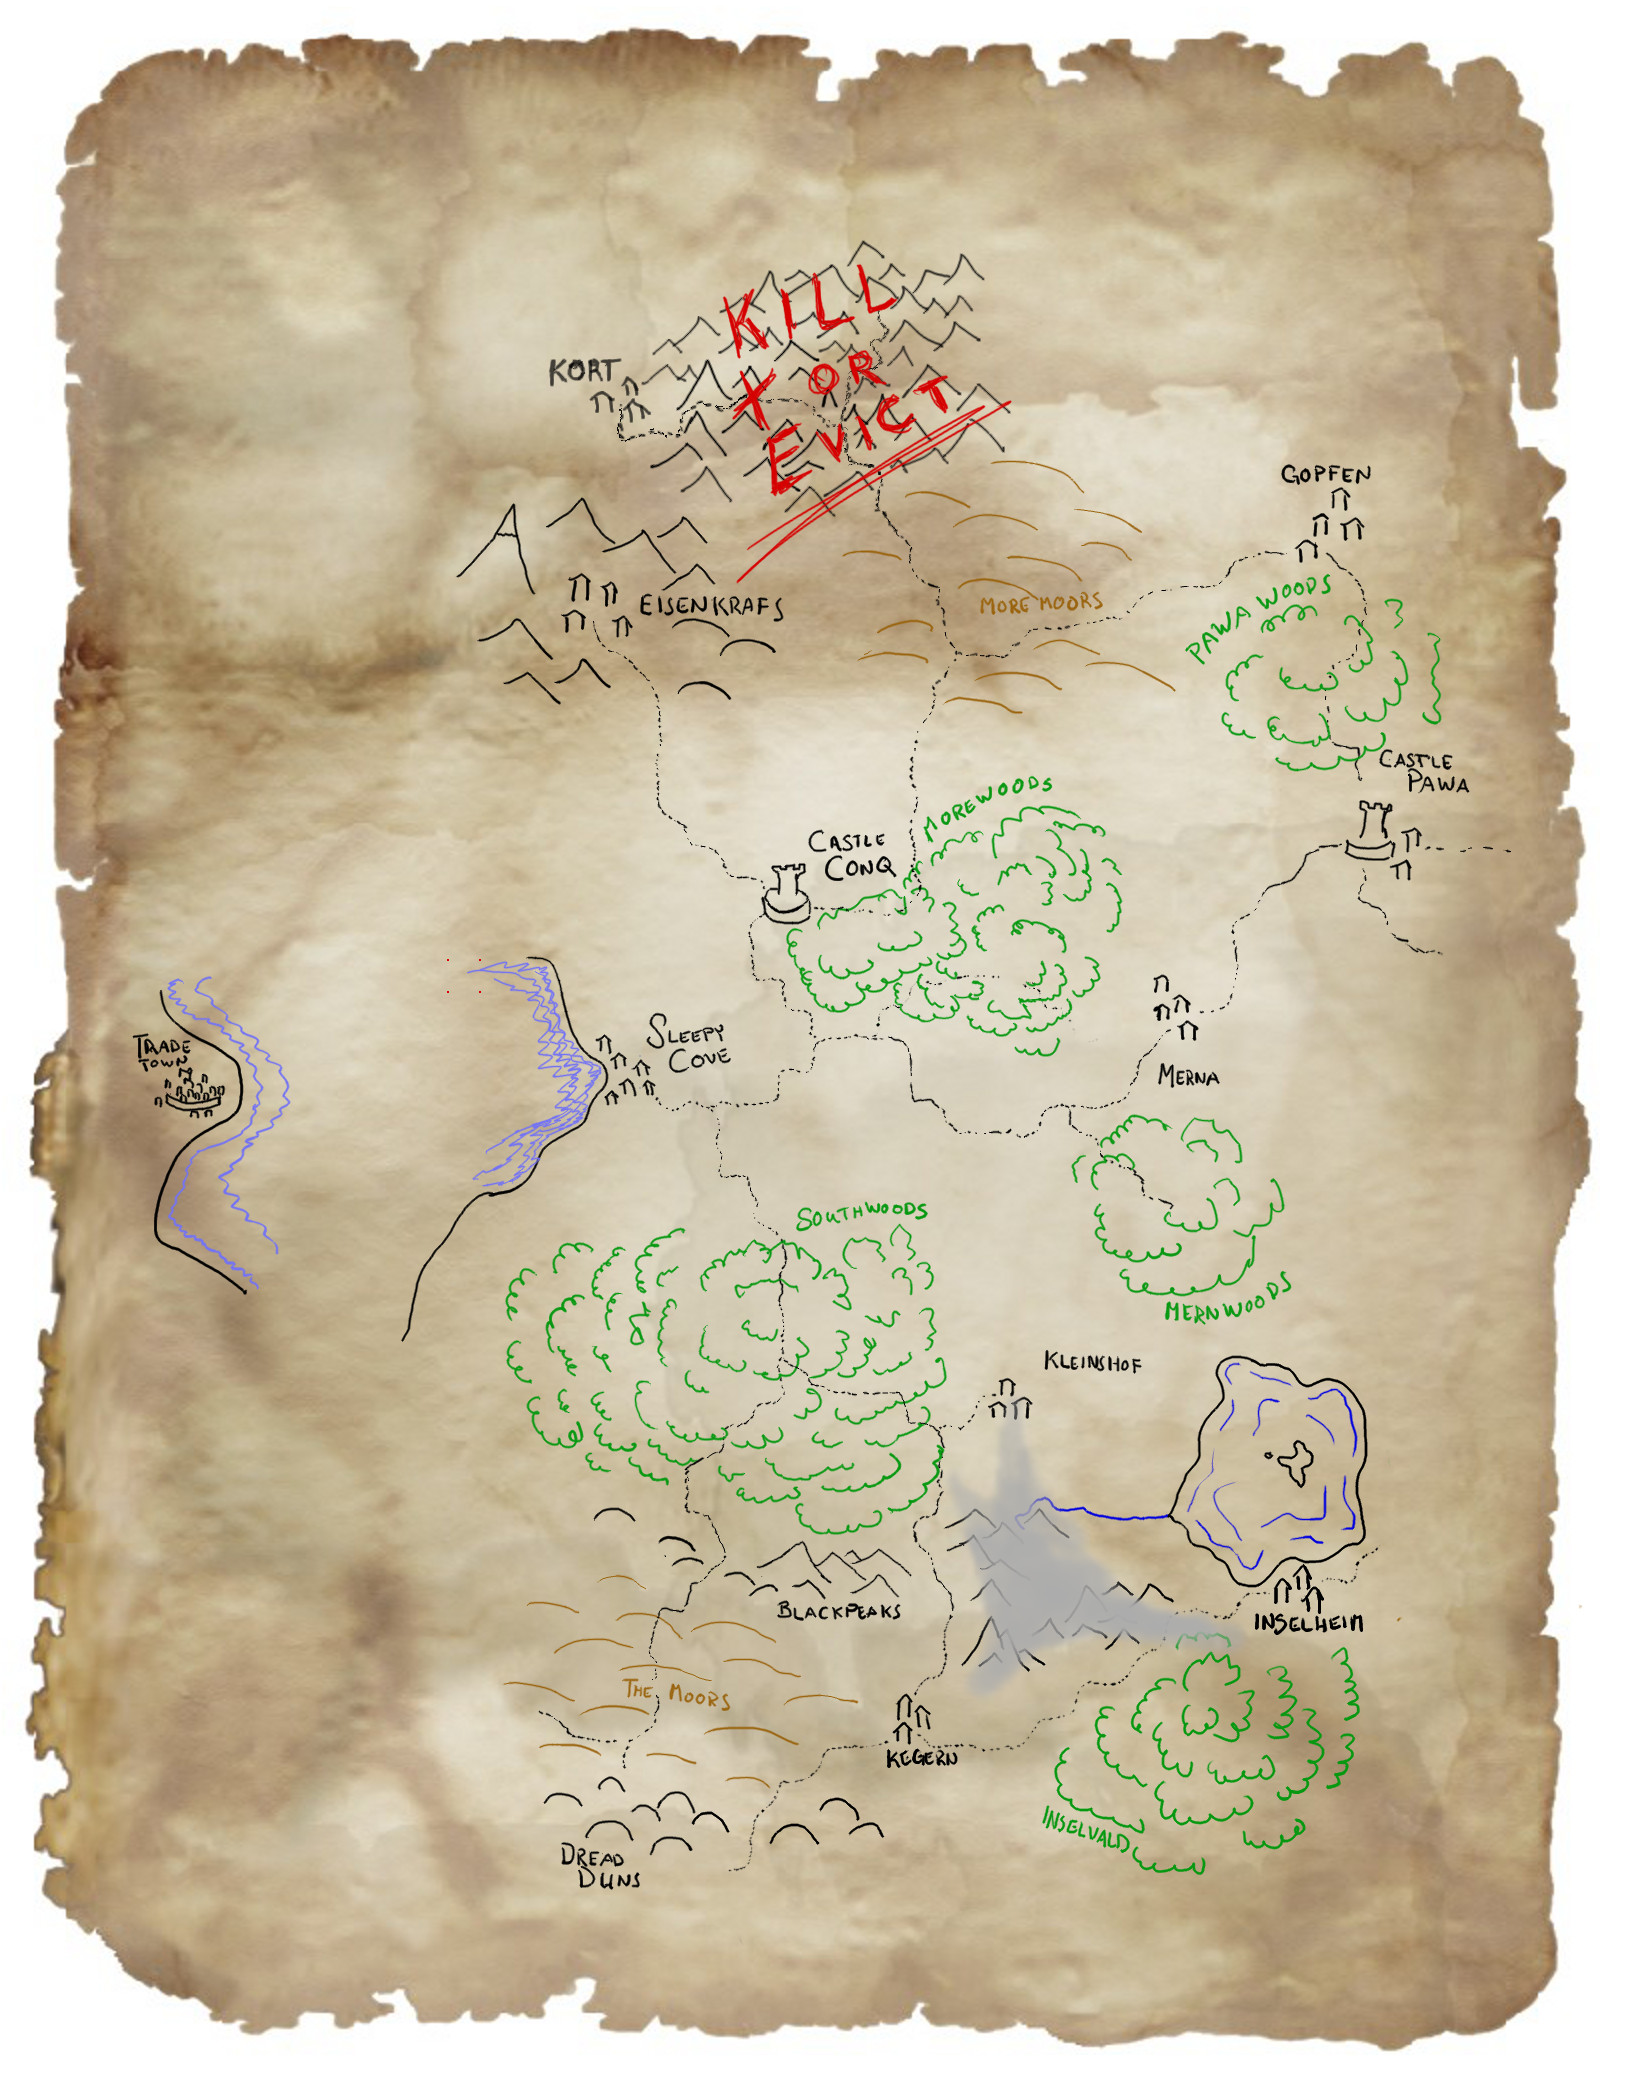
\includegraphics[width=0.999\textwidth]{./map/region-eviction-pl.jpg}
%\vfill
%\end{samepage}


%% GM map
%\clearpage                  % right opposing page
%\begin{samepage}
%\null
%\thispagestyle{empty}
%\vfill
%\noindent
%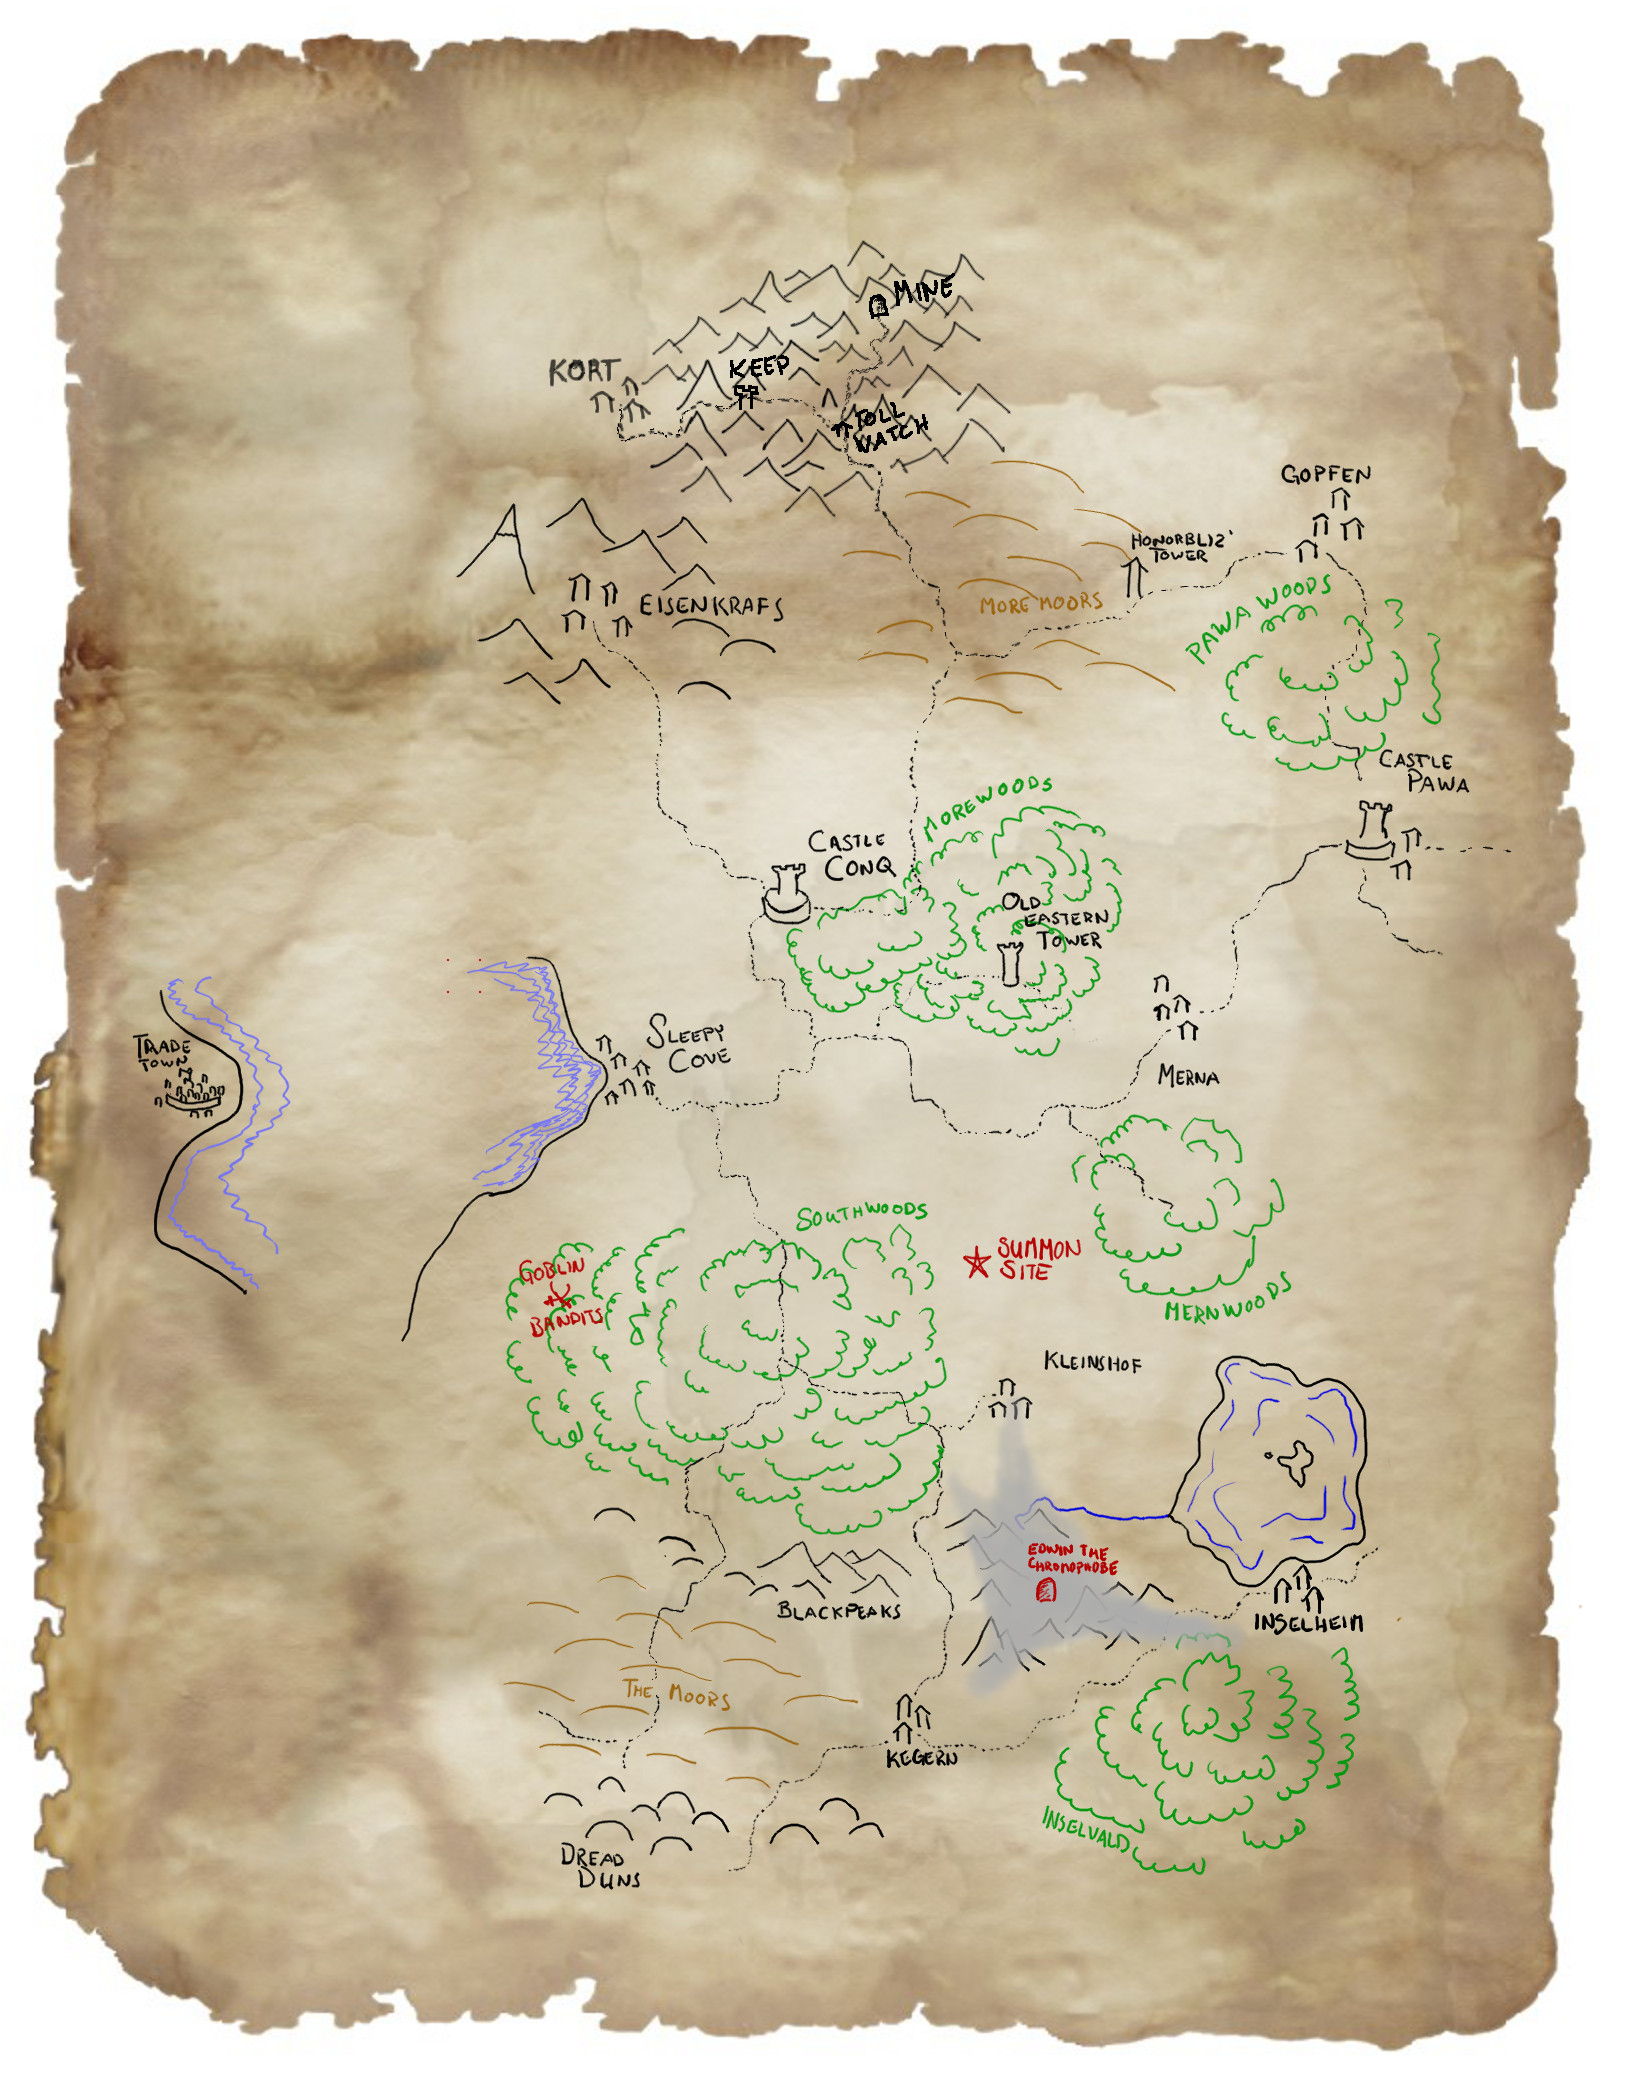
\includegraphics[width=0.999\textwidth]{./map/region-eviction-gm.jpg}
%\vfill
%\end{samepage}










%-------------------------------------------------------------------------------
% fig centered vertically on the rest of final page ?
%----------------------------------------------------
%\vfill
%\noindent
%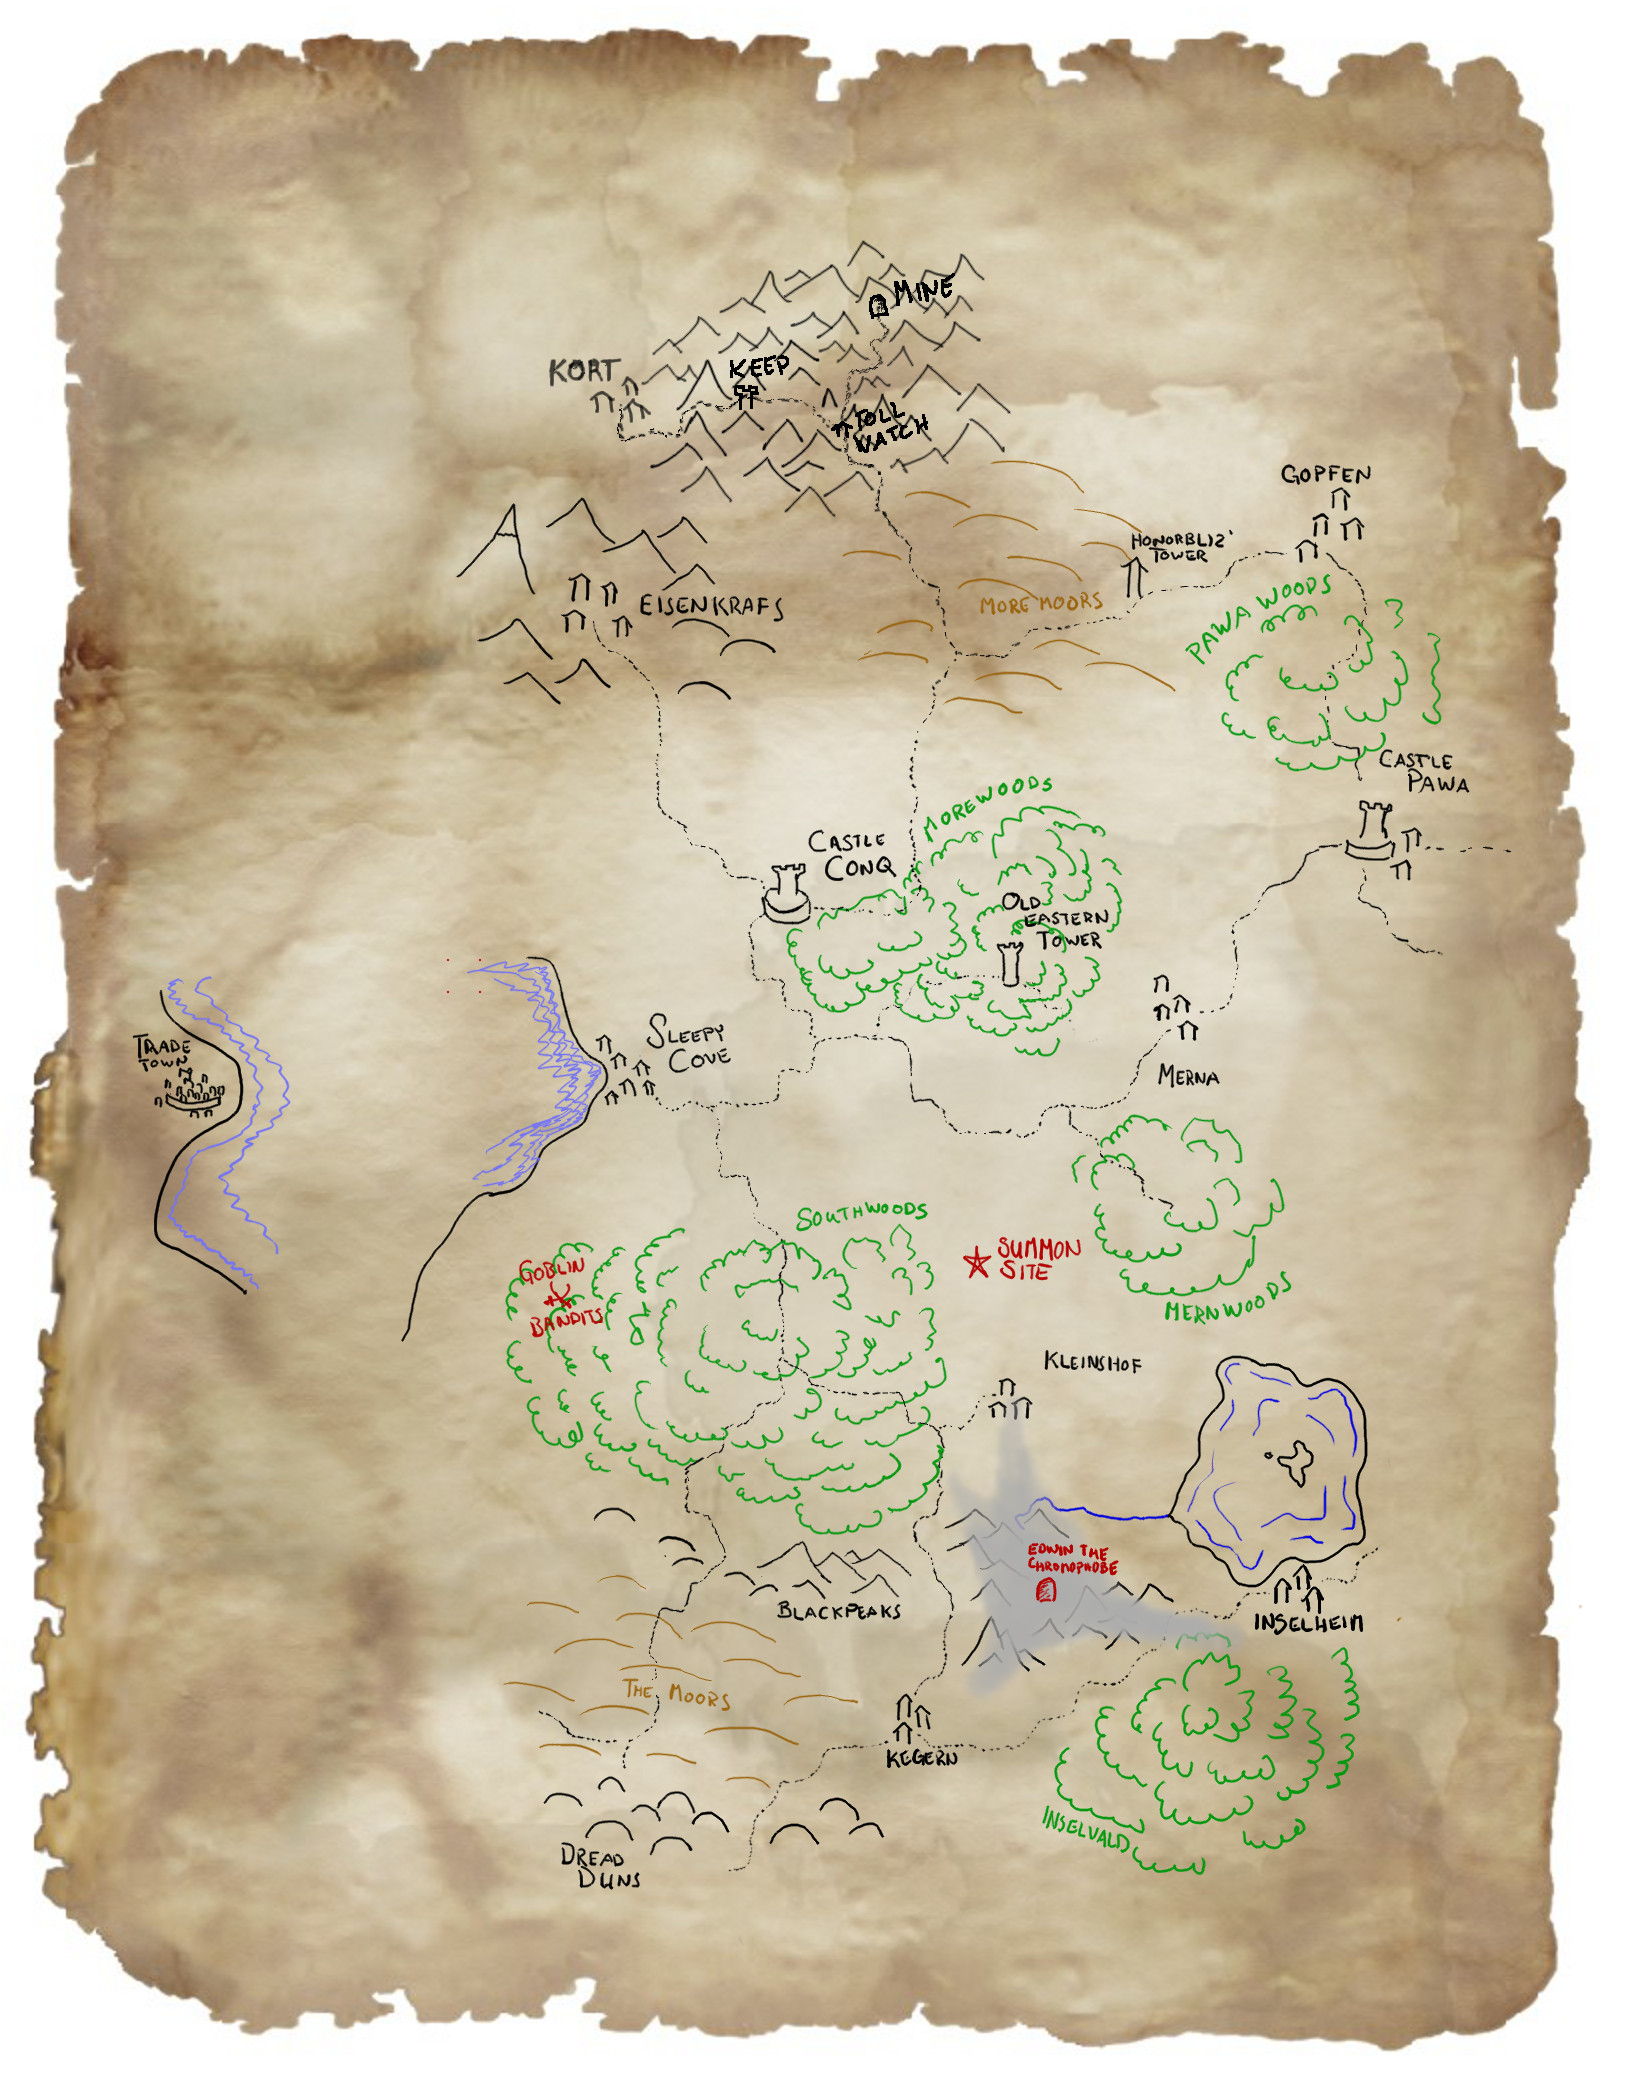
\includegraphics[width=0.999\textwidth]{./map/region-eviction-gm.jpg}
%\vfill






%-------------------------------------------------------------------------------
\end{document}
